\documentclass[a4paper]{article}
\usepackage[polish]{babel}
\usepackage[T1]{fontenc}
\usepackage[utf 8]{inputenc}
\usepackage{amsmath, amsfonts}
\usepackage{geometry}
\usepackage{url}
\usepackage{graphicx}
\usepackage{caption}
\usepackage{subcaption}
\usepackage{epstopdf}
\usepackage{amsthm,mathtools}
\usepackage{bbm}
\usepackage{hyperref}
\usepackage{url}
\usepackage{comment}
\usepackage{enumerate}
\setlength{\parindent}{0pt}
\setlength{\parskip}{1ex plus 2ex}
\pagestyle{empty}
\newgeometry{tmargin=2cm, bmargin=2cm, lmargin=2.5cm, rmargin=2.5cm}
\newtheorem{theorem}{Lemat}

\begin{document}

\begin{center}
\LARGE
\textbf{Pracownia z Analizy Numercznej (M)}\\
\end{center}
\begin{center}
\Large
Sprawozdanie do zadania \textbf{P3.5}\\
Mateusz Basiak\\
nr indeksu: 300487\\
Wrocław, 17.01.2019r.\\
\end{center}
\Large
\textbf{1.Wstęp}\\\\
\normalsize
Równania różniczkowe zwyczajne znajdują rozliczne zastosowania, zarówno w technice, jak i fizyce i matematyce. Te pierwszego rzędu są najlepiej poznane i często najprostsze, ale mimo to nie da się ich często rozwiązać analitycznie. W takich sytuacjach należy sięgnąć do metod numerycznych. Ze względu na ważne zastosowania istotne jest, by metody te były możliwie najbardziej dokładne. W tej pracy pokażę dwa często używane w przybliżeniach wzory -  Adamsa-Bashfortha i Adamsa-Moultona i przeanalizuję doświadczalnie ich dokładność.\\


\Large
\textbf{2. Opis teoretyczny}\\\\
\large
\textbf{2.1. Równania różniczkowe zwyczajne pierwszego rzędu}\\\\
\normalsize
Formalnie, rozwiązanie równania różniczkowego zwyczajnego pierwszego rzędu to rozwiązanie \textbf{zagadnienia Cauchy'ego} \cite{UW} znalezienia takiej funkcji $g(s)$, że $g(s_0) = g_0$ oraz zachodzi:
\begin{equation}\label{Cauchy}
\cfrac{dg}{ds} = F(s, g)
\end{equation}
gdzie F jest zadaną funkcją zależną od $s$ oraz $g(s)$.\\

Zdefiniujmy sobie teraz dla zadanego przedziału $[t, t+h]$ oraz stałej $b$ prostokąt R na płaszczyźnie $\mathbb{R} \times \mathbb{R}$ argumentów funkcji F jako:
\begin{equation}
R = [t, t+h] \times \{ y : |y - g_0| \leq b \} 
\end{equation}
Jest to zbiór punktów o odciętych z przedziału $[t, t+h]$, oraz rzędnych odległych od $g_0$ o co najwyżej $b$. Dalej zdefiniujmy M jako supremum funkcji $g$ na prostokącie R:  $M = sup_{(s,g) \in R} |g(s)|$\\

Załóżmy teraz, że $\cfrac{\delta F}{\delta g}$ oraz $F$ są ciągłe w prostokącie $R$. Z twierdzeń Peano i Picarda-Lindel{\H o}fa wynika wtedy od razu, że rozwiązanie zagadnienia Cauchy'ego istnieje na odcinku $[t, t+a]$ (gdzie $a = min(h, \frac{b}{M})$) i jest na nim wyznaczone jednoznacznie. \cite{UW}\\

Zauważmy, że gdy $b$ rośnie do nieskończoności, prostokąt R zamienia się w podpłaszczyznę $[t, t+h] \times \mathbb{R}$ płaszczyzny $\mathbb{R} \times \mathbb{R}$. Wtedy M staje się supremum $|g(s)|$ na przedziale $[t, t+h]$. Dodatkowo $\frac{b}{M}$ również rośnie wówczas do niekończoności, czyli $a = h$. Oznacza to, że powyższy argument przyjmuje wtedy postać:
\begin{theorem}
Jeśli funkcje $F$ oraz $\cfrac{\delta F}{\delta s}$ są ciągłe na przedziale $[t, t+h]$ zmiennej s, to zagadnienie Cauchy'ego \eqref{Cauchy} ma na nim jednoznaczne rozwiązanie.
\end{theorem}

\large
\textbf{2.2. Związek równań różniczkowych z kwadraturami}\\\\
\normalsize
W dalszej części rozważań będę brał pod uwagę tylko funkcje $F(s,g)$ ciągłe o pierwszej pochodnej ciągłej. Z poprzedniego podrozdziału wiemy, że gwarantuje to, że istnieje jednoznaczne rozwiązanie zadanego równania różniczkowego.\\
Skoro już ustaliliśmy, że równanie \eqref{Cauchy} ma jednoznaczne rozwiązanie na przedziale $[s_0, s_0+h]$, to spróbujmy je znaleźć. Całkując je obustronnie w tym przedziale otrzymujemy:
$$\int\limits_{s_0}^{s_0+h} \cfrac{dg}{ds} ds = g|_{s_0}^{s_0+h} = g(s_0+h) - g(s_0) = g(s_0+h) - g_0 = \int\limits_{s_0}^{s_0+h} F(s,g) ds$$
Zauważmy, że $h$ jest zmienną wolną w naszym równaniu, otrzymujemy więc wzór na funkcję $g$ w dowolnym punkcie $s = s_0 + h$:
\begin{equation}\label{eq}
g(s) = g(s_0+h) = g_0 + \int\limits_{s_0}^{s_0+h} F(s,g) ds
\end{equation}
Do rozwiązania brakuje nam tylko umiejętności policzenia całki $\int_{s_0}^{s_0+h} F(s,g) ds$. Bezpośrednim wnioskiem z twierdzenia Peano jest, że zagadnienie Cauchy'ego ma rozwiązanie wtedy i tylko wtedy, gdy da się policzyć tą całkę. Założyliśmy jednak wcześniej, że funkcja ta jest ciągła, a skoro liczymy całkę oznaczoną, to funkcja ta jest ograniczona, a więc jest całkowalna.\\

Niestety, mimo że dowiedliśmy, że funkcja $F$ jest całkowalna, całka ta nie zawsze jest możliwa do policzenia analitycznie. W tym miejscu należy odwołać się do metod numerycznych. Załóżmy, że chcemy wyznaczyć funkcję $g$ na pewnym określonym przedziale. Jeśli weźmiemy wówczas zbiór równoodległych punktów ${s_1, s_2, \cdots, s_n}$ i obliczmy wartość $g(s_i)$ dla każdego $i \in \{1, \cdots, n \} $ to będzie można aproksymować funkcję $g$ jako przechodzącą przez te punkty. Jeśli zbiór tych punktów będzie odpowiednio gęsty, to przybliżenie to będzie bardzo dokładne.\\
Pozostaje więc problem obliczenia całki z $F(s,g)$ na pewnym konkretnym przedziale $[s_i, s_i + h]$. Tu z pomocą przychodzą nam kwadratury typu Newtona-Cotesa, a konkretnie metody Adamsa-Bashfortha i Adamsa-Moultona.\\

\large
\textbf{2.3. Kwadratura Adamsa-Bashfortha}\\\\
\normalsize
Załóżmy, że obliczyliśmy już wartości $g$ dla punktów $s_1, s_2, \cdots, s_{i-1}$. Zdefiniujmy $h$ jako odległość między dwoma sąsiednimi punktami $s_j$ oraz $s_{j-1}$. Chcemy teraz obliczyć $g(s_i)$. Mamy więc:
$$g(s_{i+1}) = g(s_i) +  \int\limits_{s_i}^{s_{i+1}} F(s,g) ds$$
Zauważmy, że skoro znamy wartość $g$ w jakimś punkcie $s_j$, oraz mamy dany wzór jawny funkcji $F$ zależnej od $g$ oraz $s$, to można szybko obliczyć wartość funkcji $F(s_j, g(s_j))$. Do obliczenia powyższej całki można użyć wzoru Adamsa-Bashfortha \cite{KI} postaci:
\begin{equation}\label{coeff}
\int\limits_{s_i}^{s_{i+1}} F(s,g) ds = h\Bigl(A_0F(s_i,g(s_i)) + A_1F(s_{i-1},g(s_{i-1})) + \cdots\Bigr) = h\sum_{k=0}^{\infty}A_kF(s_{i-k},g(s_{i-k}))
\end{equation}
Można go teraz ograniczyć do czterech składników, uzyskując przybliżenie:
$$\int\limits_{s_i}^{s_{i+1}} F(s,g) ds \approx h\sum_{k=0}^{3}A_kF(s_{i-k},g(s_{i-k}))$$
Pozostaje znaleźć współczynniki $A_0, A_1, A_2, A_3$. Wyznaczymy je tak, aby wartość tej całki była dokładna, gdy F jest wielomianem zmiennej $t$ stopnia co najwyżej 3. Oczywiście wystarczy, by tą własność miały wielomiany z bazy tej przestrzeni (każdy wielomian to kombinacja wielomianów bazowych, więc jest to prosty wniosek z rozdzielności operacji całkowania względem dodawania). Wybierzmy więc bazę:
\begin{equation}\label{poly}
\begin{cases}
p_0(s) = 1\\
p_n(s) = \prod_{j=0}^{n-1} (s+j), \quad \quad n>0
\end{cases}
\end{equation}
Pierwsze cztery wielomiany tego ciągu tworzą bazę, choćby dlatego że są różnych stopni, więc są liniowo niezależne. Zbiór czterech liniowo niezależnych elementów przestrzeni czterowymiarowej jest bazą.\\
Obliczanie całek na przedziale $[s_i, s_{i+1}]$ jest dość niewygodne, dlatego posłużę się następującym lematem.
\begin{theorem}
Jeśli wzór:
\begin{equation} \label{lemmaa}
\int\limits_0^1f(x)dx \approx \sum_{k=-i}^0 A_i f(i)
\end{equation}
jest dokładny dla każdego $f \in \prod_3$, to tę samą własność ma wzór:
\begin{equation}\label{lemmab}
\int\limits_a^{a+h} f(x)dx \approx h\sum_{k=-i}^0 A_i f(a+ih)
\end{equation}
\end{theorem}
\begin{proof}
$$\int\limits_a^{a+h} f(x)dx =| \stackrel{dy=dx}{y=x-a}| = \int\limits_0^h f(y)dy = |\stackrel{dz=dy}{z=\frac{1}{h}y} | = h \int\limits_0^1 f(z)dz \approx$$
$$\approx h\sum_{k=-i}^0 A_i f(a+ih)$$
W ostatniej równości $f(a+ih)$ wynika z faktu, że jeśli $z$ wynosi $i$, to zgodnie z podstawieniem $y = zh = ih$, natomiast $x = a+y = a+ih$.
\end{proof}
Mając ten lemat możemy zapisać całki, dla których nasze przybliżenie ma być dokładne:
$$\int\limits_0^1 p_n(s) ds = A_0p_n(0) + A_1p_n(-1) + A_2p_n(-2) + A_3p_n(-3)$$
Rozpisując takie równania dla czterech możliwych wartości $n$ i obliczając wartości $p_n$ otrzymujemy układ czterech równań, z którego można wyliczyć interesujące nas współczynniki:
$$\begin{cases}
A_0 + A_1 + A_2 + A_3 = 1\\
-A_1 -2A_2 -3A_3 = \cfrac{1}{2}\\
2A_2 + 6A_3 = \cfrac{5}{6}\\
-6A_3 = \cfrac{9}{4}
\end{cases}$$
Po rozwiązaniu tego układu otrzymujemy współczynniki: $A_0 = \cfrac{55}{24}, A_1 = -\cfrac{59}{24}, A_2 = \cfrac{37}{24}, A_3 = -\cfrac{3}{8}$. Ostatecznie dostajemy więc wzór Adamsa-Bashfortha:
\begin{equation}\label{AB}
\int\limits_{s_i}^{s_{i+1}} F(s,g) ds \approx \cfrac{h}{24}\Bigl(55F(s_ig(s_i)) - 59F(s_{i-1},g(s_{i-1})) + 37F(s_{i-2},g(s_{i-2})) - 9F(s_{i-3},g(s_{i-3}))\Bigr)
\end{equation}
Jest to kwadratura rzędu cztery.\\

\large
\textbf{2.4. Kwadratura Adamsa-Moultona}\\\\
\normalsize
Zauważmy, że we wzorze Adamsa-Bashfortha wartość $g(s_{i+1})$ nie zależy od wartości funkcji $F$ w tym punkcie. Może to powodować niedokładności. Dlatego często stosuje się go razem ze wzorem Adamsa-Moultona \cite{KI}, który ma taką samą postać jak wzór \eqref{coeff}, rozszerzony o jeden składnik na początku:
\begin{equation}
\int\limits_{s_i}^{s_{i+1}} F(s,g) ds = h\sum_{k=-1}^{\infty}A_kF(s_{i-k},g(s_{i-k}))
\end{equation}
Oczywiście do obliczenia wartości $F(s_{i+1}, g(s_{i+1})$ musimy już znać wartość $g(s_{i+1})$, dlatego najpierw zastosujemy wzór Adamsa-Bashfortha do uzyskania pewnego jej przybliżenia, a potem z pomocą wzoru Adamsa-Moultona je poprawimy.\\
Ponownie jak w przypadku poprzedniego wzoru, ograniczmy go do czterech składników, uzyskując kwadraturę rzędu cztery. \textbf{Lemat 2} nadal ma tu zastosowanie. Możemy również skorzystać z bazy wyznaczonej wcześniej \eqref{poly}. Otrzymujemy równanie: 
$$\int\limits_0^1 p_n(s) ds = A_{-1}p_n(1) + A_0p_n(0) + A_1p_n(-1) + A_2p_n(-2)$$
Ponownie z czterech takich równań po podstawieniu wartości wielomianów $p_n$ otrzymujemy układ równań:
$$\begin{cases}
A_{-1} + A_0 + A_1 + A_2 = 1\\
A_{-1} -A_1 -2A_2 = \cfrac{1}{2}\\
2A_{-1} + 2A_2= \cfrac{5}{6}\\
6A_{-1} = \cfrac{9}{4}
\end{cases}$$
Z którego otrzymujemy współczynniki: $A_{-1} = \cfrac{9}{24}, A_0 = \cfrac{19}{24}, A_1 = -\cfrac{5}{24}, A_2 = \cfrac{1}{24}$. Ostatecznie kwadratura ta ma postać:
\begin{equation}\label{AM}
\int\limits_{s_i}^{s_{i+1}} F(s,g) ds \approx \cfrac{h}{24}\Bigl(9F(s_{i+1}, g(s_{i+1}) + 19F(s_ig(s_i)) - 5F(s_{i-1},g(s_{i-1})) + F(s_{i-2},g(s_{i-2}))\Bigr)
\end{equation} 

\large
\textbf{2.5. Wzory Rungego-Kutty}\\\\
\normalsize
Ostatnim problemem jest fakt, że we wzorze \eqref{AB} używamy wartości $g(s_i), g(s_{i-1}), g(s_{i-2}), g(s_{i-3})$. Na początku działania naszego algorytmu, do wyliczenia $g(s_4)$ będą nam więc potrzebne $g(s_3), g(s_2), g(s_1), g(s_0)$, a tylko ta ostatnia jest dana w założeniach. Należy więc z jak najlepszym przybliżeniem znaleźć trzy pierwsze wartości $g$. Jest na to kilka sposobów. Jednym z nich jest metoda Rungego-Kutty rzędu czwartego. \cite{KI} \cite{WI} Jest ona dobrze udokumentowana w źródłach, a jej dowód jest dość prosty i nie jest częścią zadania, dlatego go pominę i ograniczę się do podania wzorów:
\begin{equation}\label{RK}
g(s_0 + kh) \approx g(s_0) + \cfrac{1}{6}(G_1 + 2G_2 + 2G_3 + G_4)
\end{equation}
$$\begin{cases}
G_1 = khF(s_0, g(s_0))\\
G_2 = khF(s_0 + \frac{1}{2}kh, g(s_0) + \frac{1}{2}G_1)\\
G_3 = khF(s_0 + \frac{1}{2}kh, g(s_0) + \frac{1}{2}G_2)\\
G_4 = khF(s_0 + kh, g(s_0) + G_3)\\
\end{cases}$$
Ze wzoru \eqref{RK} można obliczyć wszystkie trzy potrzebne współczynniki.\\\\

\Large
\textbf{3. Opis programu}\\\\
\normalsize
Wszystkie doświadczenia wykonywane były za pomocą programu zaimplementowanego w języku Julia v.1.0.1. Program ten uruchamiano na komputerze z procesorem Intel Core i5, 1.60GHz, 4 GB RAM, długość słowa maszynowego 64 bit. Precyzja arytmetyki to $u = 1,11 \cdot 10^{-16}$. Program, umieszczony w pliku $"program.jl"$, składa się z następujących funkcji:
\begin{description}
\item[$algorithm(F, s_0, g_0, l, n)$] \hfill\\ Główna funkcja algorytmu. Wywołuje ona pozostałe funkcje z odpowiednimi argumentami. Przyjmuje ona argumenty: $F$ - funkcja $F(s, g)$; $s_0$ - początek przedziału; $l$ - jego długość; $n$ - liczba równoodległych punktów tworzących podział odcinka $[s_0, s_0 + l]$, w których należy policzyć wartość funkcji $g$; $g_0$ - wartość $g(s_0)$. Funkcja zwraca tablicę rozmiaru $n+1$ z obliczonymi wartościami funkcji $g$ w kolejnych punktach.
\item[$Runge\_Kutta(F, s_0, g_0, kh)$] \hfill\\ Funkcja pomocnicza obliczająca przybliżoną wartość $g(s_0 + kh)$ metodą Rungego-Kutty.
\item[$next\_point(F, h, s_1, F0, F1, F2, F3, g_0)$] \hfill\\ Funkcja obliczająca przybliżoną wartość funkcji $g$ w punkcie $s_1$ wzorami Adamsa-Bashfortha i Adamsa-Moultona. Argumenty $F0, F1, F2, F3$ to wartości funkcji $F(s,g)$ odpowiednio w punktach $(s_i, g(s_i)), (s_{i-1}, g(s_{i-1})), (s_{i-2}, g(s_{i-2})), (s_{i-3}, g(s_{i-3}))$, argument $g_0$ to wartość $g(s)$ w punkcie $s_1 - h$.
\item[$Adams\_Bashforth(h, F0, F1, F2, F3)$] \hfill\\ Funkcja pomocnicza implementująca wzór Adamsa-Bashfortha.
\item[$Adams\_Moulton(h, F\_1, F0, F1, F2)$] \hfill\\ Funkcja pomocnicza implementująca wzór Adamsa-Moultona.
\end{description}
\newpage



\Large
\textbf{4. Doświadczenia}\\\\
\normalsize
Jako że zadanie, polegające na obliczaniu całki, ma w założeniu być tylko częścią większego algorytmu numerycznego obliczania funkcji $g(s)$, skupię się na sprawdzaniu dokładności tego ostatniego. Na początek jednak przetestuję na kilku prostych funkcjach dokładność obliczania całek.\\

\large
\textbf{4.1. Dokładność funkcji $Adams\_Bashforth$ i $Adams\_Moulton$}\\\\
\normalsize
Zacznijmy od przetestowania samych funkcji bazujących na wzorach $Adamsa-Bashfortha$ i $Adamsa-Moultona$ dla kilku podstawowych funkcji $F$. Dla każdej z nich mogę obliczyć ręcznie wynik i porównać go z tym otrzymanym z zastosowania tych wzorów.
\begin{center}
\large
\textbf{Wzór Adamsa-Bashfortha}

\normalsize
$\begin{tabular}{|c|c|c|c|c|} 
\hline
{Funkcja F} & {Przedział } & {Wynik dokładny} & {Wynik otrzymany} & {Błąd względny} \\ \hline
\begin{math}
F_1 = x^2 - 3x + 10
\end{math} &
[-1, 2] &
28.5 & 28.5 & 0.0 \\ \hline
\begin{math}
F_2 = x^3 - 7x^2 - 13x + 28
\end{math} &
[-10,10] & -4106.7 & -4106.666667 & 0.000008 \\ \hline
\begin{math}
F_3 = cos(x)
\end{math} &
\begin{math}
 [ \cfrac{-\pi}{2} , \cfrac{\pi}{2} ]
\end{math} & 
2 & 0.000000 & 1.0 \\ \hline
\begin{math}
F_4 = x \cdot 3^{2x^2 + 3}
\end{math} &
[0,2] &
\begin{math}
\cfrac{54}{ln 3} \approx 49.152918238
\end{math} &
\begin{math}
1.87823 \cdot 10^{247}
\end{math} &
\begin{math}
3.8212 \cdot 10^{245} 
\end{math} \\ \hline
\begin{math}
F_5 = \begin{cases}
x^2 - 2 \quad \quad \quad \quad \quad x \leq -2\\
2x^3 + 4x^2 - 7 \quad -2 < x \leq 1\\
5x^2 - 3x - 1 \quad \quad \quad x > 1\\
\end{cases}
\end{math} &
[-5,5] & 
\begin{math}
183\cfrac{1}{6} \approx 183.166667
\end{math} & 
63.333333 & 0.654231 \\ \hline
\begin{math}
F_6 = x^6 - 6x^4 + 10x + 30
\end{math} &
[3, 10] & 1309215.6 & -69498115.166667 & 54.083782 \\ \hline
\end{tabular}$
\hfill
\break

\large
\textbf{Wzór Adamsa-Moultona}

\normalsize
$\begin{tabular}{|c|c|c|c|c|} 
\hline
{Funkcja F} & {Przedział } & {Wynik dokładny} & {Wynik otrzymany} & {Błąd względny} \\ \hline
\begin{math}
F_1 = x^2 - 3x + 10
\end{math} &
[-1, 2] &
28.5 & 28.5 & 0.0 \\ \hline
\begin{math}
F_2 = x^3 - 7x^2 - 13x + 28
\end{math} &
[-10,10] & -4106.7 & -4106.666667 & 0.000008 \\ \hline
\begin{math}
F_3 = cos(x)
\end{math} &
\begin{math}
 [ \cfrac{-\pi}{2} , \cfrac{\pi}{2} ]
\end{math} & 
2 & 0.000000 & 1.0 \\ \hline
\begin{math}
F_4 = x \cdot 3^{2x^2 + 3}
\end{math} &
[0,2] &
\begin{math}
\cfrac{54}{ln 3} \approx 49.152918238
\end{math} &
\begin{math}
-1.79289 \cdot 10^{97}
\end{math} &
\begin{math}
3.64758 \cdot 10^{95} 
\end{math} \\ \hline
\begin{math}
F_5 = \begin{cases}
x^2 - 2 \quad \quad \quad \quad \quad x \leq -2\\
2x^3 + 4x^2 - 7 \quad -2 < x \leq 1\\
5x^2 - 3x - 1 \quad \quad \quad x > 1\\
\end{cases}
\end{math} &
[-5,5] & 
\begin{math}
183\cfrac{1}{6} \approx 183.16667
\end{math} & 
385.833333 & 1.106460 \\ \hline
\begin{math}
F_6 = x^6 - 6x^4 + 10x + 30
\end{math} &
[3, 10] & 1309215.6 & 2956861.83333 & 1.258499 \\ \hline
\end{tabular}$
\end{center}


Z powyższych doświadczeń wynika jasno, że wzory Adamsa-Bashfortha i Adamsa-Moultona nie dają dobrych rezultatów dla dowolnych funkcji $F(x)$. W szczególności, jak wynika z doświadczeń dla funkcji $F_1$ i $F_2$ są one dokładne dla funkcji należących do $\prod_3$. Obserwacja ta jest zgodna z założeniami dotyczącymi rzędu tych kwadratur. Dla pozostałych funkcji, jak pokazuje np. przykład $F_4$, oba wzory mogą dawać bardzo duże błędy, choć wzór Adamsa-Moultona jest precyzyjniejszy. Warunek ciągłości $g(x)$ (jak i jej pierwszej pochodnej), który cały czas zakładaliśmy w naszych rozważaniach również okazuje się istotny, co pokazuje przykład $F_5$. Funkcja ta jest funkcją sklejaną nieciągłą, której części należą do $\prod_3$, ale błąd względny jej obliczania jest znacząco większy niż dla $F_1$ i $F_2$, a błąd bezwzględny jest rzędu wyniku.\\

\large
\textbf{4.2. Wyznaczanie rozwiązań równań różniczkowych zwyczajnych pierwszego rzędu}\\\\
\normalsize
W tej części zbadamy, jak dokładny jest cały algorytm, wyznaczający funkcję $g(s)$ na podstawie funkcji $F(s,g)$, korzystający ze wzorów Adamsa-Bashfortha, Adamsa-Moultona i Rungego-Kutty. Aby wyniku nie zakłócały niedokładności, które zaobserwowaliśmy w rozdziale 4.1., będziemy rozważali wyłącznie takie funkcje $F$, które są wielomianem dwóch zmiennych $s$ oraz $g$ i sumaryczny stopień obu zmiennych w pojedynczym składniku tego wielomianu nie przekracza trzech.\\
Zauważmy przy tym, że w żadnym miejscu nie czynimy założeń na temat funkcji $g(s)$ (poza tym, że istnieje ona na zadanym przedziale), więc nie musi ona być wielomianem.\\
Jako że rozwiązywanie analityczne równań różniczkowych nie jest przedmiotem tej pracy, będziemy posługiwali się przykładami równań zamieszczonymi w literaturze. \cite{UW}\\

\large
\textbf{4.2.1. $F(s,g) = g$}\\\\
\normalsize
Na początek weźmy funkcję $F(s,g) = g$,  oraz przedział [0,3]. Ustalmy $g(0) = 2$. Wówczas rozwiązaniem równania jest $g(s) = 2e^s$.

\begin{figure}[h!]
  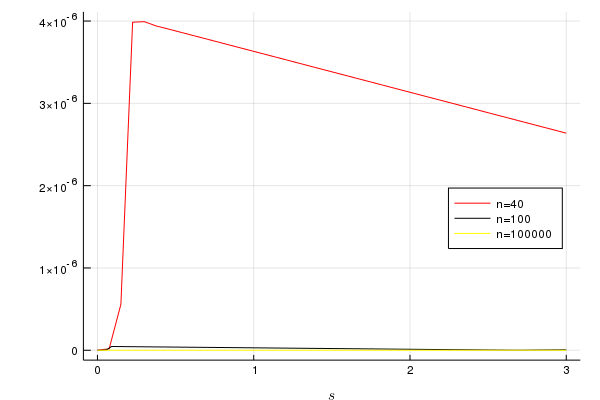
\includegraphics[width=11cm]{F1_error.png}
  \caption{Błąd względny obliczania wartości funkcji g(s)}
\end{figure}

Na wykresie pokazany jest błąd względny przybliżenia $g(s)$, a nie wykres samej funkcji i jej przybliżenia, gdyż te dwa ostatnie leżą zbyt blisko siebie i taki wykres byłby nieczytelny. Z ryciny powyżej widać, że błąd względny przybliżenia maleje  bardzo szybko w zależności od zagęszczenia punktów, w których funkcja $g(s)$ jest przybliżana. Dla $n=100$ maksymalny błąd przybliżenia na tym przedziale wynosi  $4.56556 \cdot 10^{-8}$, zaś dla $n=100000$ już tylko $2.94667 \cdot 10^{-14}$.\\

\large
\textbf{4.2.2. $F(s,g) = g(5-g)$}\\\\
\normalsize
Rozważmy równanie $F(s,g) = g(5-g)$ na przedziale [0,2] dla warunku początkowego $g(0) = 1$. Jego rozwiązaniem jest $g(s) = 5 \cdot \cfrac{e^{5s}}{4 + e^{5s}}$.

\begin{figure}[h!]
  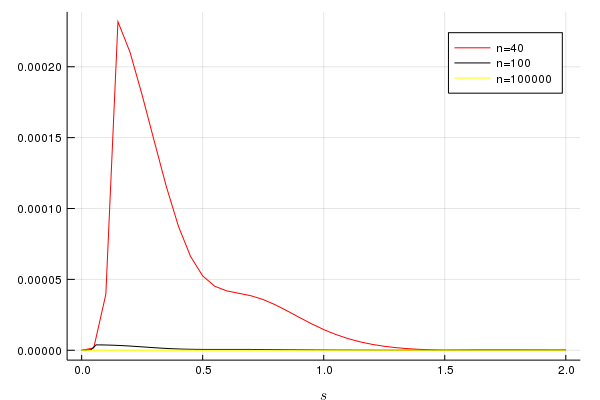
\includegraphics[width=11cm]{F2_error.png}
  \caption{Błąd względny obliczania wartości funkcji g(s)}
\end{figure}

Na powyższym wykresie ponownie błąd dla $n=40$ jest znacząco większy od pozostałych. Jest on rzędu $10^{-4}$, co może już poważnie zakłócać wynik. Tak duże rozbieżności w porównaniu do poprzedniego przykładu mogą wynikać np. z bardziej skomplikowanej formy funkcji $g(s)$, czy z wyższego stopnia wielomianu $F(s,g)$. Jednak zwiększanie liczby punktów węzłowych przybliżenia pozwala wygładzić wykres i w konsekwencji znacząco zmniejszyć błąd przybliżenia. Dla $n=100000$ jest on równy maksymalnie $8.05046 \cdot 10^{-15}$, czyli zaledwie jeden rząd wielkości więcej, niż precyzja arytmetyki. Jest to bardzo dobre przybliżenie i świadczy o dużej precyzji zarówno algorytmu, jak i jego implementacji.\\

\large
\textbf{4.2.3. $F(s,g) = g^3$}\\\\
\normalsize
Rozważmy równanie $F(s,g) = g^3$ na przedziale [1,10] dla warunku początkowego $g(1) = \cfrac{1}{ \sqrt{20}}$. Jego rozwiązaniem jest $g(s) = \cfrac{1}{ \sqrt{2(11-s)}}$.

\begin{figure}[h!]
  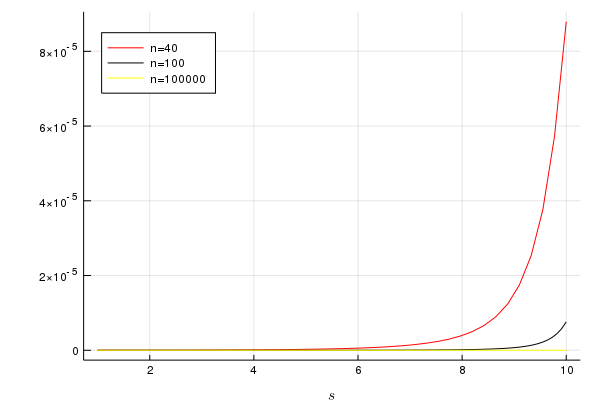
\includegraphics[width=11cm]{F3_error.png}
  \caption{Błąd względny obliczania wartości funkcji g(s)}
\end{figure}

Zauważmy, że zarówno funkcja $g(s)$, jak i $F(s,g)$ są bardzo małe przy początku badanego przedziału, lecz potem rosną coraz szybciej w kierunku jego końca. Dlatego również błąd, początkowo będąc bliski precyzji arytmetyki nawet przy niewielkim zagęszczeniu punktów węzłowych, rośnie bardzo szybko. Mimo to dla $n=100000$ wzrost $g(s)$ udało się opanować i przybliżenie pozostało precyzyjne, jego maksymalny błąd względny wyniósł $4.85834 \cdot 10^{-14}$.\\

\Large
\textbf{5.Wnioski}
\normalsize

Wzory Adamsa-Bashfortha i Adamsa-Moultona są przydatne do rozwiązywania równań różniczkowych zwyczajnych pierwszego rzędu. Mimo, że nie są one zawsze dokładne, to dla pewnej klasy funkcji (wielomiany stopnia co najwyżej o jeden mniejszego, niż stopień tych kwadratur, które nie są funkcjami sklejanymi) dają bardzo precyzyjne wyniki. Jeśli funkcja $F$ należy do tej klasy, to przy użyciu odpowiednio wielu (rzędu 100000) punktów węzłowych, algorytm bazujący na tychże wzorach przybliża $g$ z precyzją bliską precyzji arytmetyki. Dzieje się tak niezależnie od skompikowania funkcji $g$. Jest to więc bardzo dobre narzędzie do rozwiązywania tego typu problemów i może być z powodzeniem używane w praktyce.

\newpage
\begin{thebibliography}{9}
\itemsep2pt

\bibitem{UW} F. Przytycki, Równania Różniczkowe Zwyczajne, skrypt, Uniwersytet Warszawski, 2001 \url{https://www.mimuw.edu.pl/~radamcz/teaching/skrypt.pdf}

\bibitem{KI} W.Cheney, D. Kincaid, Numerical mathematics and computing, sixth edition, Brooks/Cole: Cengage Learning, 2007

\bibitem{WI} Za Wikipedią: \url{https://en.wikipedia.org/wiki/Runge%E2%80%93Kutta_methods#Second-order_methods_with_two_stages}

\end{thebibliography}

\end{document}